\documentclass[11pt,letterpaper]{article}
\usepackage[latin1]{inputenc}
\usepackage{amsmath}
\usepackage{amsfonts}
\usepackage{amssymb}
\usepackage{url}
\usepackage{graphicx}
\author{J. Decker}
\date{26 Feb 2012}
\title{Ground Test of xBee Radios}
\begin{document}
\maketitle
\begin{abstract}
A range test was attempted without success.  The setup and test results are discussed, and recommendations for future ground tests are given.
\end{abstract}

\section{Objective and Success Criteria}
\begin{description}
\item[Objective:] Demonstrate the conservative useful range of xBee Pro radios and 2dBi antennas.
\item[Success Criteria:] Transmit and receive packets at 466 meters range; observe received signal strength indication of the base radio.
\end{description}

\section{Setup}
A significant amount of time was spent getting the remote xBee radio to simply echo data back to the base xBee.  It was found that by removing the xBee radio from the prototyping breadboard and placing it in a dedicated carrier board (either the Adafriut or Sparkfun USB board), a successful loop-back test could be achieved.

The hardware setup consisted of two xBee radios: a base unit and a remote unit.  The base unit was seated on Sparkfun's USB breakout board and made use of Digi's X-CTU software \footnote{\url{http://www.digi.com/support/productdetail?pid=3352&osvid=57&type=cabling}} running on a Windows PC.  The software continually sends a message of 32-bytes to the remote unit.  The remote xBee was seated on Adafruit's xBee adpater	\footnote{\url{http://www.ladyada.net/make/xbee/}} and powered from a 4.5V headlamp battery \footnote{\url{http://www.amazon.com/dp/B002BZEJM2/}}. The $Data_{In}$ and $Data_{Out}$ lines of the remote xBee radio were connected.  The block diagram of the setup is shown in Figure \ref{figHardwareBlockDiagram}. 

\begin{figure}[htb]
\begin{center}
%trim=<l> <b> <r> <t>
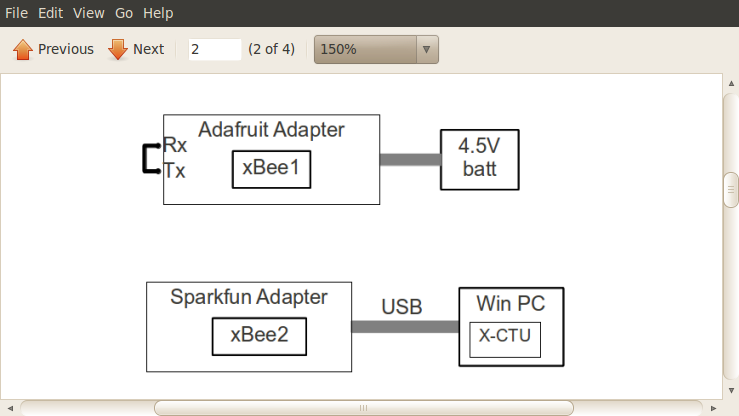
\includegraphics[scale=.6, trim = 10mm 10mm 10mm 40mm, clip]{hardwareBlockDiagram.png}
\centering
\caption{Hardware block diagram of 26 Feb 2012 ground tests.}
\label{figHardwareBlockDiagram}
\end{center}
\end{figure}

The base unit was placed in an open window as seen in Figure \ref{xbeewindow}.  The open window in the author's ``Boy Room" faced roughly northeast and allowed a clear line of sight to a convenient intersection more than 450m away.  Figure \ref{googleMaps} illustrates the distance and orientation of the range test.  According to Google Maps, the distance from the base radio to the remote radio was only 466m.


\begin{figure}[htb]
\begin{center}
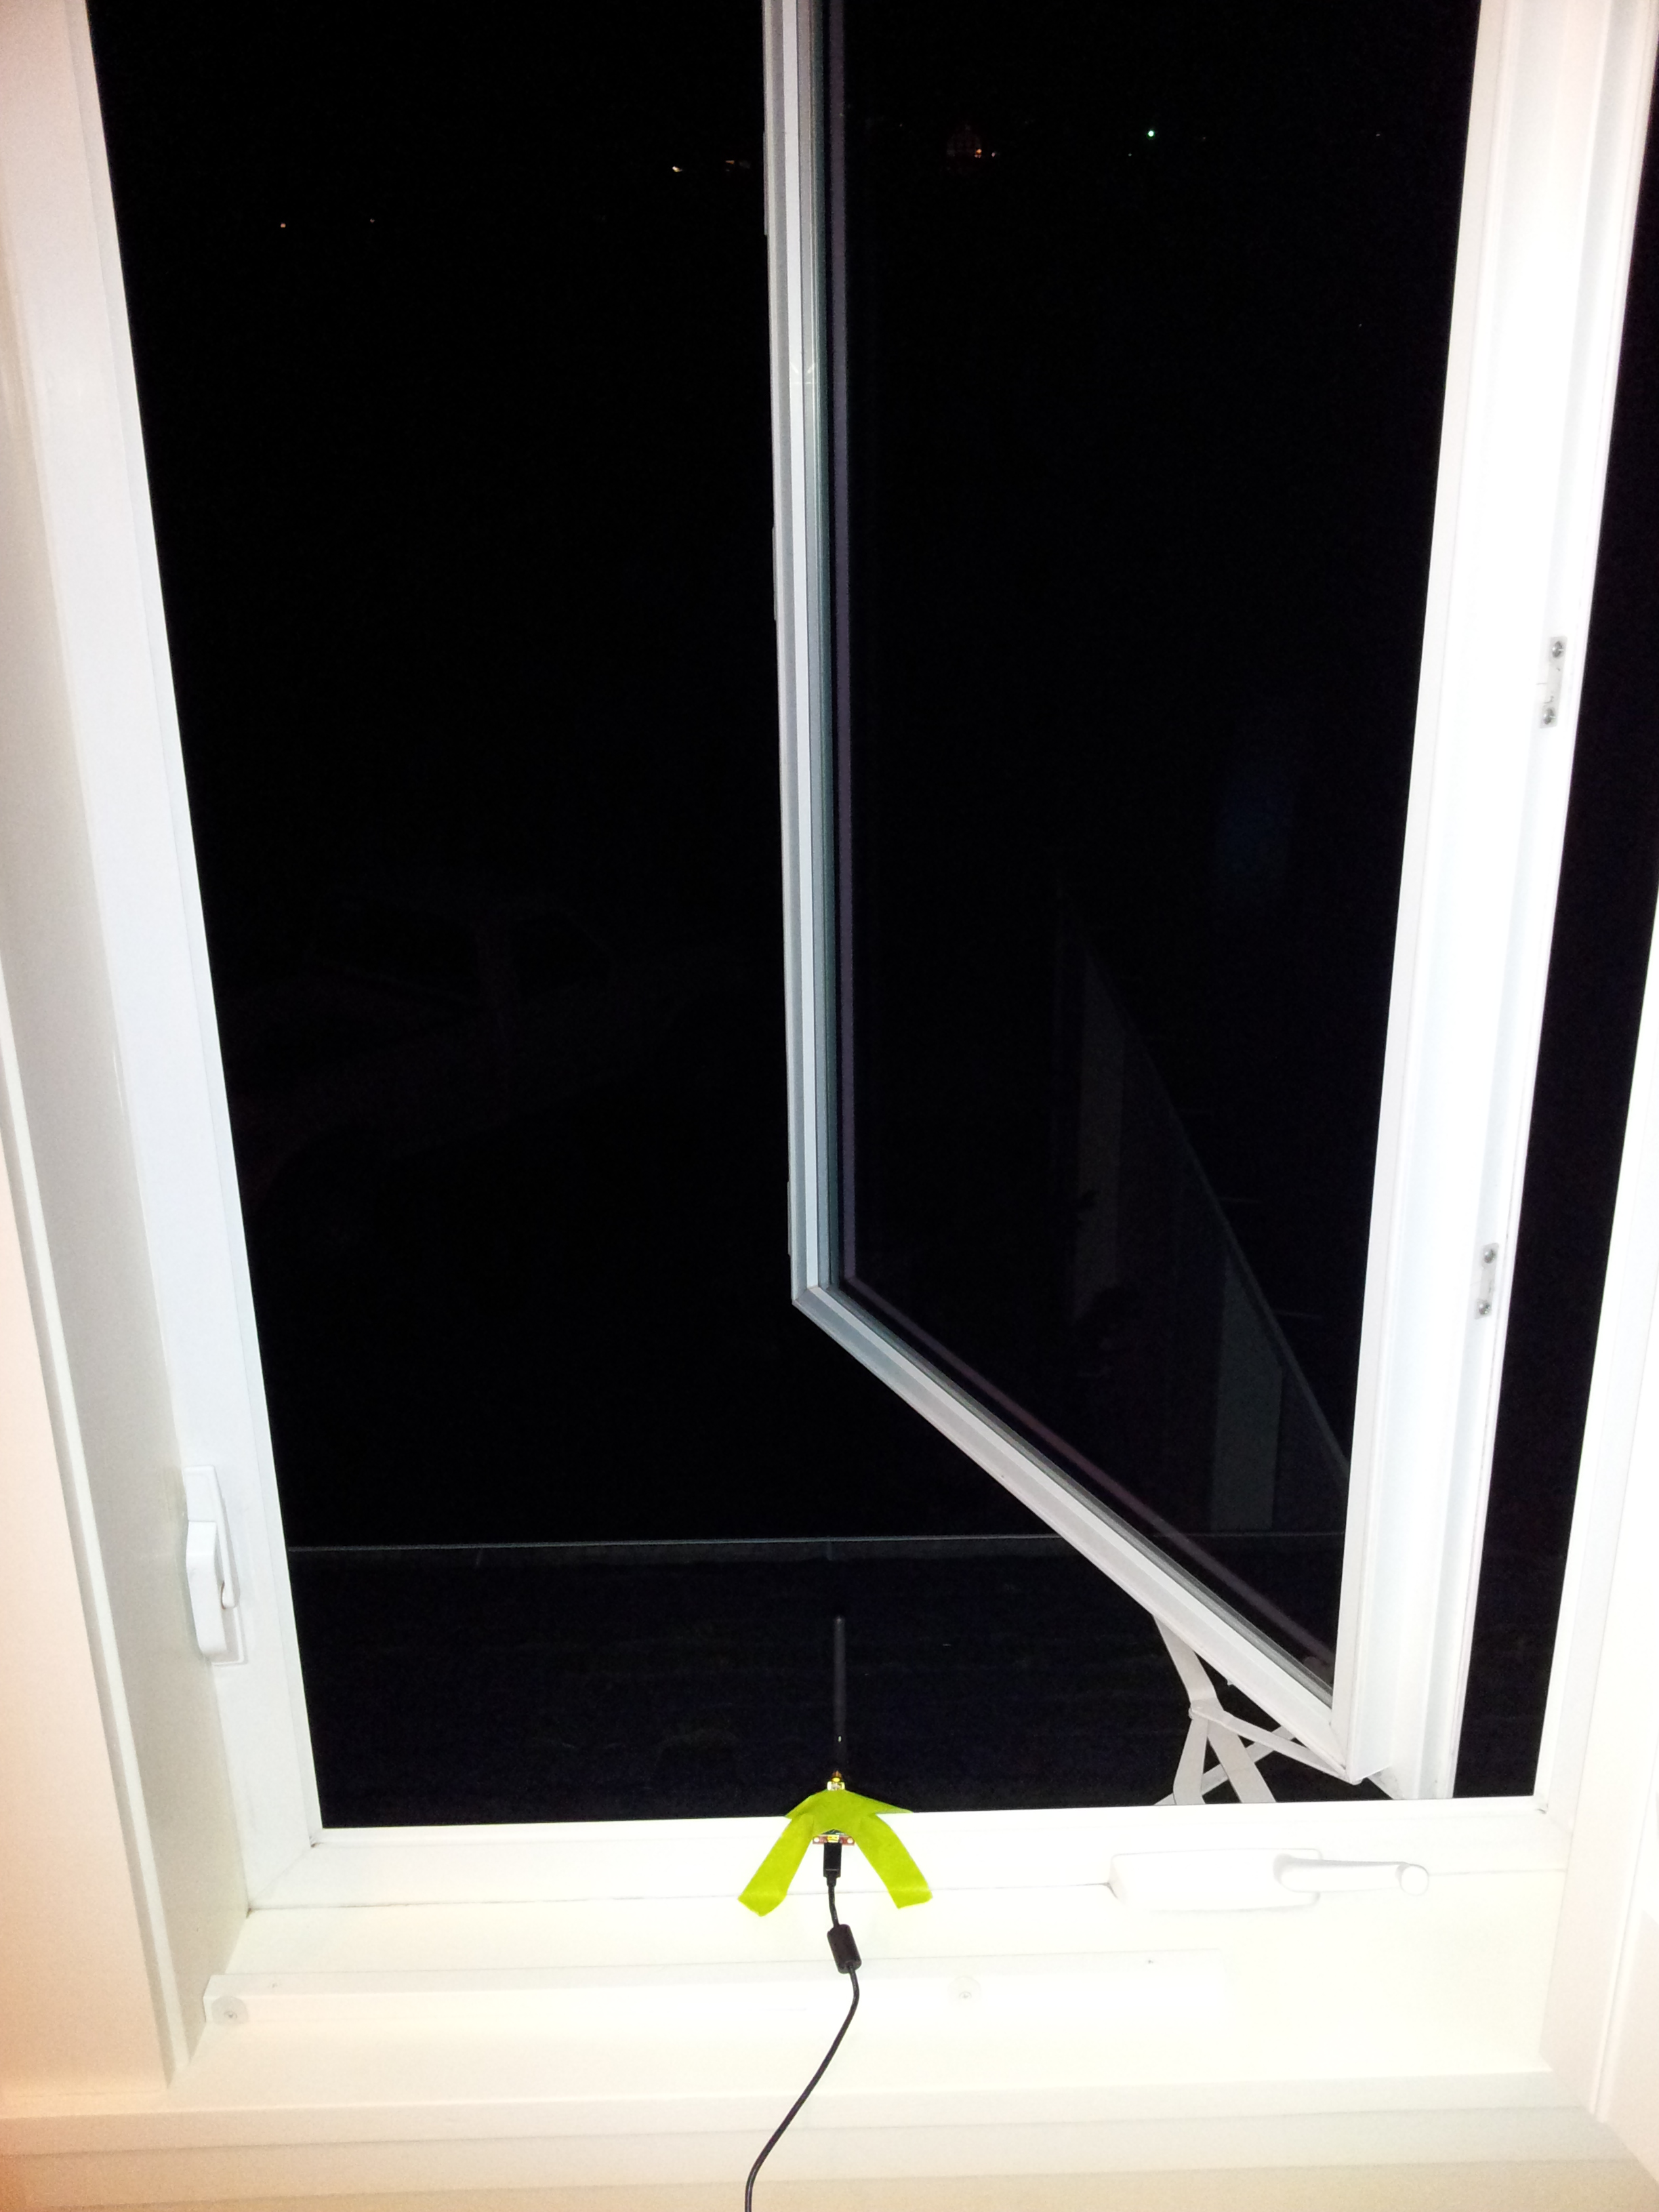
\includegraphics[scale=.1, angle = 270]{xbeeWindow.jpg}
\centering
\caption{Base radio situated in window.}
\label{xbeewindow}
\end{center}
\end{figure}

\begin{figure}[htb]
\begin{center}
%trim=<l> <b> <r> <t>
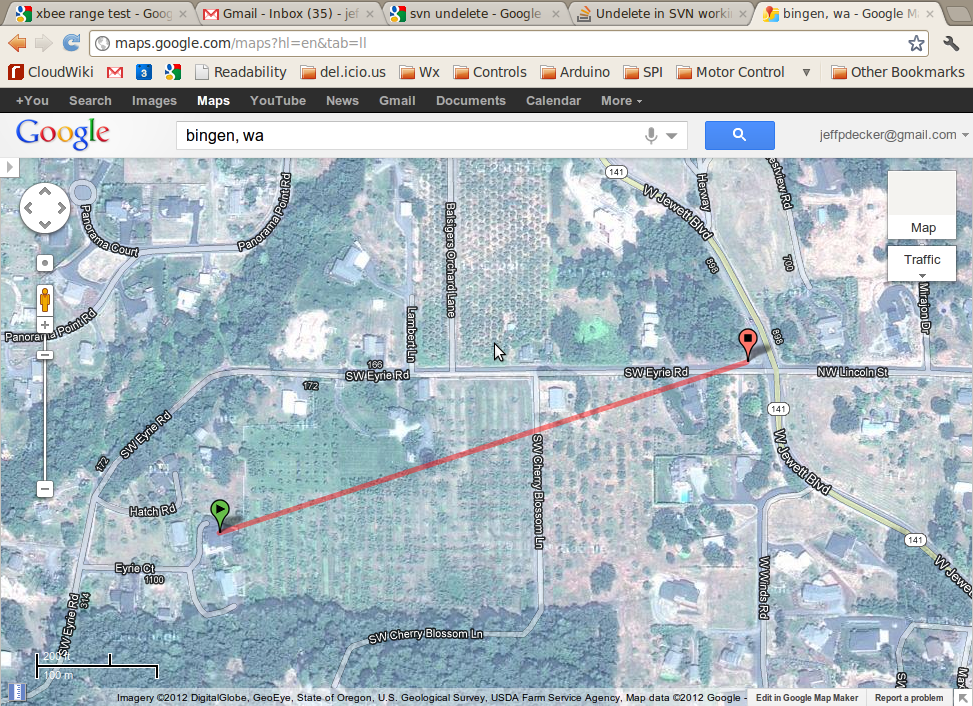
\includegraphics[scale=0.6, trim = 50mm 40mm 60mm 60mm, clip]{googleMaps.png}
\centering
\caption{Google maps view of line of sight range test.}
\label{googleMaps}
\end{center}
\end{figure}


\section{Results}
The hardware and software setup was confirmed working at a range of $\sim$5m, at a reported Received Signal Strength Indication (RSSI) of -82dB before setting out to the remote location.

At the intersection of Jewett Rd and Eyrie Rd, the remote radio was powered on and its antenna oriented vertically. The power LED and RSSI LED were confirmed on. A cellphone call (3G AT\& T, 1900MHz or 850MHz?) back to the base radio observer reported dismal performance: 3 of $\sim$200 packets were echoed back to the base radio successfully.  Interestingly, the author suffered poor cellphone reception until the xBee radio was separated from the cellphone by $\sim$10m.

\section{Analysis}
The RSSI should have been much higher at close range.  Initial hypothesis centered on not enough power being delivered  to the remote xBee radio, therefore allowing the packets to be received (the RSSI LED was on), but not allowing the transmission back to the base radio.  However, the battery voltage of the remote xBee was confirmed to at 4.1V with the remote xBee at full receive and transmit load.

Because a limited number of packets did successfully get echoed back to the base station, it's assumed the hardware setup was in fact correct.

It's possible the cellphone call interrupted the service to the xBee radio.  Because the cellphone call was initiated before the remote radio established a connection, the radio performance without the RF presence of a cellphone is not know.

\section{Recommendations}
The next range test should be arranged such that the remote xBee radio is connected via USB to a laptop running the X-CTU software.  With this arrangement, the remote radio performance can be monitored without cell phone calls back to the base radio observer.  The remote radio's performance can be established as a function of distance, instead of a binary operational check at one location.


\end{document}